% ------------------------------------------------------------------------------
% TYPO3 Version 10.3 - What's New (Dutch Version)
%
% @license	Creative Commons BY-NC-SA 3.0
% @link		https://typo3.org/help/documentation/whats-new/
% @language	Dutch
% ------------------------------------------------------------------------------

\section{Inleiding}
\begin{frame}[fragile]
	\frametitle{Inleiding}

	\begin{center}\huge{Inleiding}\end{center}
	\begin{center}\huge{\color{typo3darkgrey}\textbf{De feiten}}\end{center}

\end{frame}

% ------------------------------------------------------------------------------
% TYPO3 Version 10.3 - The Facts

\begin{frame}[fragile]
	\frametitle{Inleiding}
	\framesubtitle{TYPO3 Versie 10.2 - De feiten}

	\begin{itemize}
		\item Publicatiedatum: 25 februari 2020
		\item Publicatietype: Sprint Release
	\end{itemize}

	\begin{figure}
		
\includegraphics[width=0.95\linewidth]{Introduction/typo3-v10-3-banner.png}
	\end{figure}

\end{frame}

% ------------------------------------------------------------------------------
% TYPO3 Version 10.3 - Executive Summary

\begin{frame}[fragile]
	\frametitle{Inleiding}
	\framesubtitle{Managementsamenvatting}

	\small
		Als de laatste sprint release van de v10 cyclus is TYPO3 versie 10.3 de zogenaamde
		"\href{https://typo3.org/article/land-ho-feature-freeze-ahead}{feature freeze}"
		versie. Dit betekent: geen nieuwe functies vanaf nu tot de LTS-versie in april, en
		het core team en iedereen die bijdraagt zijn gericht op testen, oppoetsen en het
		verfijnen van deze versie.

		\vspace{0.2cm}

		Echter, er zijn wat uitzonderingen voor kleine verbeteringen aan reeds complete
		functies die al zijn toegevoegd in vorige v10 sprint versies.

		\vspace{0.2cm}

		Extensieontwikkelaars wordt verzocht versies van extensies die compatibel zijn met
		v10 te publiceren. Hierdoor kan de TYPO3 gemeenschap eenvoudiger TYPO3 v10 inzetten
		zodra de LTS-versie beschikbaar is.

		\vspace{0.2cm}

		Nog een belangrijk ding: vergeet niet naar een
		\href{https://typo3.org/community/events/v10-parties}{release party} te gaan
		of er een zelf te organiseren!

	\normalsize

\end{frame}

% ------------------------------------------------------------------------------
% System Requirements

\begin{frame}[fragile]
	\frametitle{Inleiding}
	\framesubtitle{Systeemeisen}

	\begin{itemize}
		\item PHP versie 7.2, 7.3 of 7.4
		\item PHP instellingen:

			\begin{itemize}
				\item \texttt{memory\_limit} >= 256M
				\item \texttt{max\_execution\_time} >= 240s
				\item \texttt{max\_input\_vars} >= 1500
				\item compilatieoptie \texttt{-}\texttt{-disable-ipv6} moet \underline{niet} worden gebruikt
			\end{itemize}

		\item De meeste databaseservers die worden ondersteund door \textbf{Doctrine DBAL} werken ook met TYPO3.
			De geteste database systemen zijn:
	\end{itemize}

	\begin{figure}
		
\includegraphics[width=0.80\linewidth]{Introduction/logo-databases.png}
	\end{figure}

\end{frame}

% ------------------------------------------------------------------------------
% Development, Release, and Maintenance Timeline

\begin{frame}[fragile]
	\frametitle{Introduction}
	\framesubtitle{Ontwikkeling-, versie- en onderhouds-tijdlijn}

	\textbf{TYPO3 v10}

	\begin{figure}
		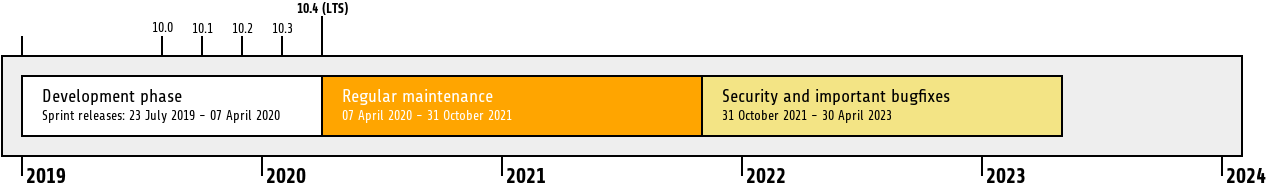
\includegraphics[width=1\linewidth]{Introduction/typo3-v10-lifecycle.png}
	\end{figure}

	\textbf{Verlengde ondersteuning}\newline
	\smaller
	De \href{https://typo3.com}{TYPO3 GmbH} biedt nog extra ondersteuningsopties aan
	voor TYPO3 v10 LTS, zelfs na 30 april 2023 tot twee jaar lang.
	\normalsize

\end{frame}

% ------------------------------------------------------------------------------
% TYPO3 v10 Roadmap

\begin{frame}[fragile]
	\frametitle{Introduction}
	\framesubtitle{TYPO3 v10 Roadmap}

	Verwachte verschijningsdata en de focus van de versie:

	\begin{itemize}

		\item v10.0 \tabto{1.1cm}23/juli/2019\tabto{3.4cm}De weg vrijmaken voor spannende nieuwe concepten en API's
		\item v10.1 \tabto{1.1cm}01/okt/2019\tabto{3.4cm}Verbeterde routing en Site behandeling v2
		\item v10.2 \tabto{1.1cm}03/dec/2019\tabto{3.4cm}Fluid/Rendering Engine verbeteringen
		\item
			\begingroup
				\color{typo3orange}
				v10.3 \tabto{1.1cm}25/feb/2020\tabto{3.4cm}Feature Freeze
			\endgroup
		\item v10.4 \tabto{1.1cm}21/apr/2020\tabto{3.4cm}LTS Release (Long-term Support)

	\end{itemize}

	\vspace{0.6cm}
	\smaller
		\url{https://typo3.org/article/typo3-v10-roadmap/}\newline
		\url{https://typo3.org/article/typo3-v10-safe-and-sound/}
	\normalsize

\end{frame}

% ------------------------------------------------------------------------------
% Installation

\begin{frame}[fragile]
	\frametitle{Inleiding}
	\framesubtitle{Installatie}

	\begin{itemize}
		\item Offici\"ele \textit{klassieke} installatieprocedure op Linux/Mac OS X\newline
		(DocumentRoot bijvoorbeeld \texttt{/var/www/site/htdocs}):
\begin{lstlisting}
$ cd /var/www/site
$ wget --content-disposition get.typo3.org/10.2
$ tar xzf typo3_src-10.2.0.tar.gz
$ cd htdocs
$ ln -s ../typo3_src-10.2.0 typo3_src
$ ln -s typo3_src/index.php
$ ln -s typo3_src/typo3
$ touch FIRST_INSTALL
\end{lstlisting}

		\item Symbolische koppelingen op Microsoft Windows:

			\begin{itemize}
				\item Gebruik \texttt{junction} op Windows XP/2000
				\item Gebruik \texttt{mklink} op Windows Vista en Windows 7 of hoger
			\end{itemize}

	\end{itemize}
\end{frame}

% ------------------------------------------------------------------------------
% Installation using composer

\begin{frame}[fragile]
	\frametitle{Installatie en Upgrade}
	\framesubtitle{Installatie met \texttt{composer}}

	\begin{itemize}
		\item Installatie met \textit{composer} onder Linux, Mac OS X en Windows 10:

\begin{lstlisting}
$ cd /var/www/site/
$ composer create-project typo3/cms-base-distribution typo3v10 ^10.3
\end{lstlisting}

		\item Of anders kan een maatwerk \texttt{composer.json} bestand gemaakt worden en dan:

\begin{lstlisting}
$ composer install
\end{lstlisting}

			Een voorbeeld \texttt{composer.json} is te downloaden van:\newline
			\smaller
				\href{https://composer.typo3.org}{https://composer.typo3.org}
			\normalsize

	\end{itemize}
\end{frame}

% ------------------------------------------------------------------------------
